

\newpage

This paper describes the development and experimental results of navigation algorithms for an autonomous underwater glider (AUG) that employs an on-board acoustic Doppler current profiler (ADCP). AUGs are buoyancy-driven autonomous underwater vehicles that uses small hydrofoils to make forward progress while profiling vertically. During each dive, which can last up to 6 hours, the Seaglider AUG used in this experiment typically reaches the depth of 1,000 m and travels 3-6 km horizontally through the water, relying solely on dead-reckoning. Horizontal through-the-water (TTW) progress of AUG is 20-30 cm/s, which is comparable to the speed of the stronger ocean currents. Underwater navigation of an AUG in the presence of unknown advection therefore presents a considerable challenge. We present a post-processing algorithm to simultaneously estimate the ocean current profile through which the AUG was flown, as well as the AUG's horizontal position as influenced by the local currents. Extensive work by Todd et al in this domain employed a modified version of the lowered ADCP estimation framework \cite{Todd2017,Todd2011}.  In addition to this estimation framework, our work uses current data from the entire dive (as opposed to just during descent) and incorporates nonlinear hydrodynamic and attitude models from the vehicle navigation system to produce a time-varying current profile for the entire dive.

Results are demonstrated using ADCP data collected from two Seaglider AUGs deployed for 49 days off the north coast of Alaska during August and September 2017. Each glider was equipped with a Nortek Signature1000 1 MHz ADCP. Figure \ref{fig.SG} shows an ADCP installed, facing upwards, in the tail section of one of the AUGs. The ADCPs are configured by Nortek to use only three beams---in the upward-facing position, those are the two side beams and the aft beam during descent, and the two side beams and the forward beam during ascent. The ADCPs were programmed to collect a profile every 15 seconds. Each profile covers up to 20 m depth, with a new profile starting approximately every 1.5 m (i.e., the vertical distance covered by the AUG in 15 seconds).

\begin{figure}[!ht]
  \centering
  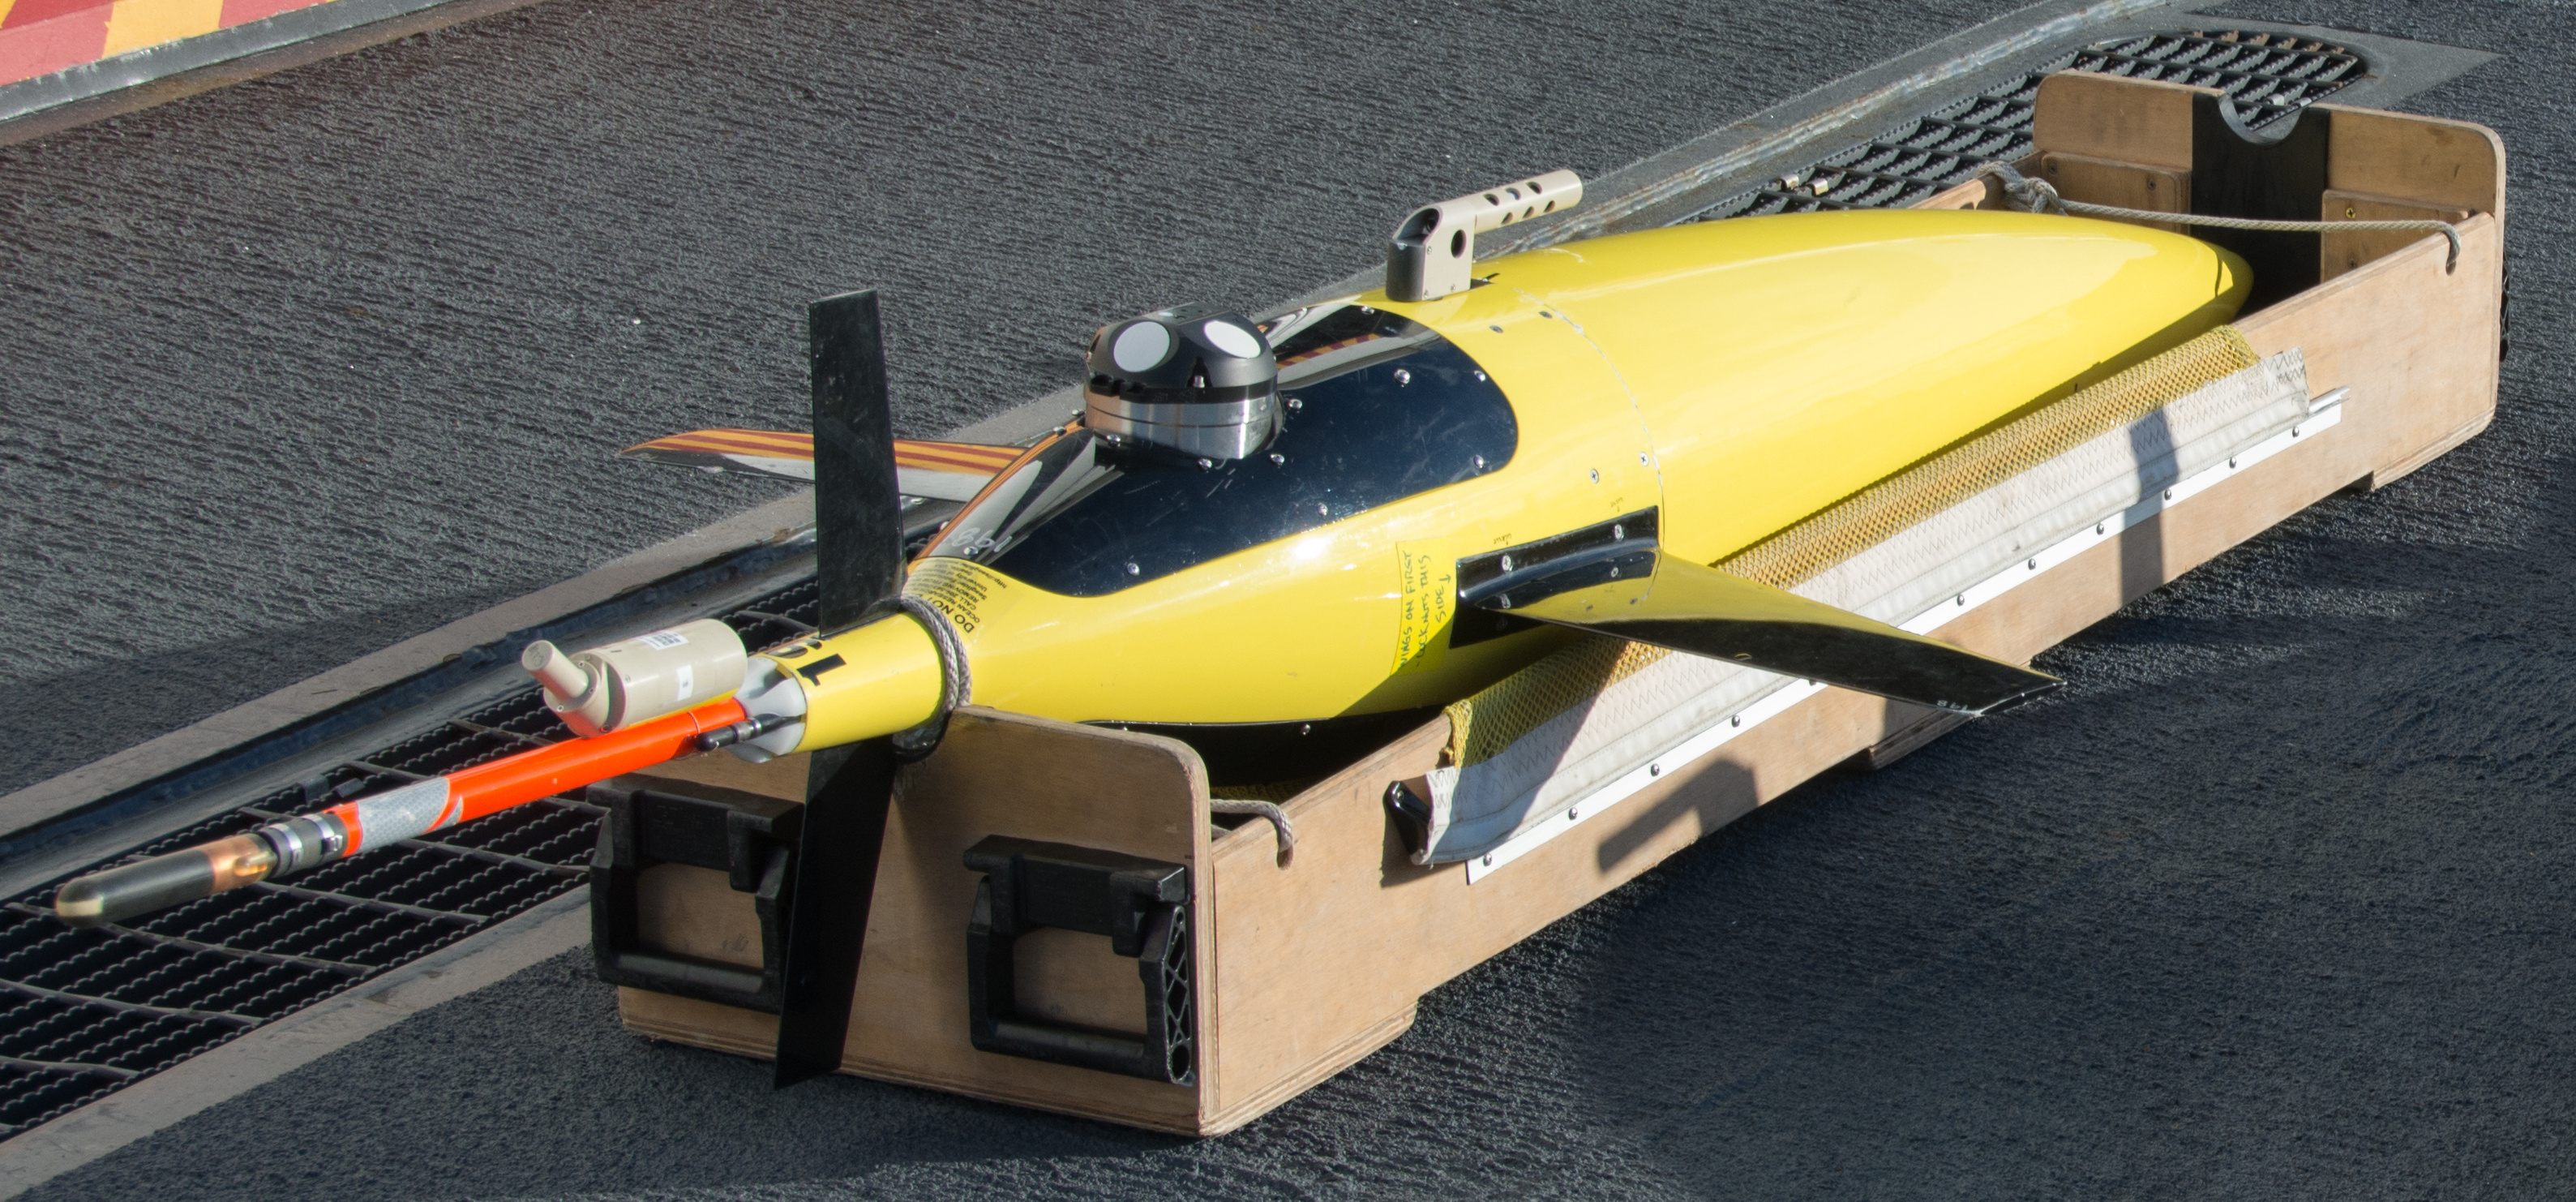
\includegraphics[width=3.0in]{./figs/Gliders_hires-99_crop.jpg}
  %\vspace{-0.1in}
  \caption{Seaglider AUG with an upwards-facing ADCP installed in aft fairing.}
  \label{fig.SG}
%   \vspace{-0.1in}
  %\rule{\textwidth}{0.02in}
  \vspace{-0.2in}
\end{figure}

The main challenge of AUG-based ADCP velocity profiling is that each velocity profile is measured relative to the TTW motion of the glider, which is generally unknown. TTW velocity can be inferred from the AUG dynamic model, but is subject to uncertainty because the model is based on steady state flight and doesn't take roll into account. This lack of a georeferenced platform velocity produces the need to perform a simultaneous robust estimation of current and glider TTW velocity using all available data -- ADCP velocity profiles, surrounding water density, glider buoyancy engine state, glider attitude and angle of attack, glider depth, and GPS positions at the start and end of the dive. Figure 2 shows a short section of the dive with the individual ADCP profiles, offset by our initial estimate of the AUG's TTW velocity (i.e., the velocity from the hydrodynamic model, without accounting for current-induced motion). The thick black line is the estimated current profile. This is from a 750 m dive, so the sections of data shown were collected 3.5 hrs apart. The difference in the current profile during ascent and descent are clearly visible, motivating the need for different current profiles during ascent and descent.

\begin{figure}[!ht]
  \centering
  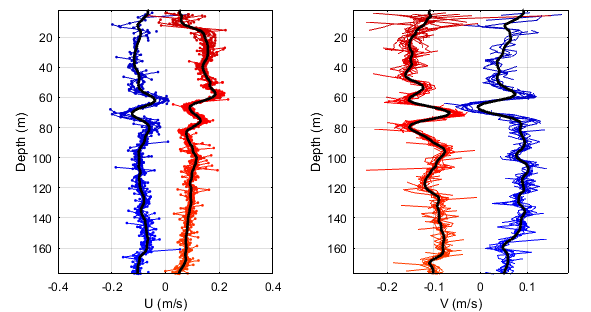
\includegraphics[width=\columnwidth]{./figs/current_profile_snip.png}
  \vspace{-0.1in}
  \caption{ Overlapped ADCP profiles during descent (blue) and ascent (red) for dive 116 of sg198. The fitted current profile is shown as the thick black line.}
  \label{fig.profile_snip}
   \vspace{-0.1in}
  %\rule{\textwidth}{0.02in}
%   \vspace{-0.2in}
\end{figure}

\begin{thebibliography}{1}

\bibitem{Todd2017}
Todd, R.E., D.L. Rudnick, J.T. Sherman, W.B. Owens, L. George, Absolute velocity estimates from autonomous underwater gliders equipped with Doppler current profilers, \emph{J. Atmos. Oceanic Technol.}, 34(2), 309–333.%, doi:10.1175/JTECH-D-16-0156.1.

\bibitem{Todd2011}
Todd, R.E., D.L. Rudnick, M.R. Mazloff, R.E. Davis, B.D. Cornuelle, Poleward flows in the southern California Current System: Glider observations and numerical simulation, \emph{J. Geophys. Res.}, 116, C02026. %, doi:10.1029/2010JC006536.

\end{thebibliography}
